\subsection{\large{Хранилище расчётных данных}}
\addcontentsline{toc}{subsection}{Хранилище расчётных данных}

Детальная архитектура хранилища расчётных данных представлена на диаграмме компонент
(см. рис\ \ref{pic:architecture__storage-component}).

\begin{figure}[H]
	\hspace*{-2.5 cm}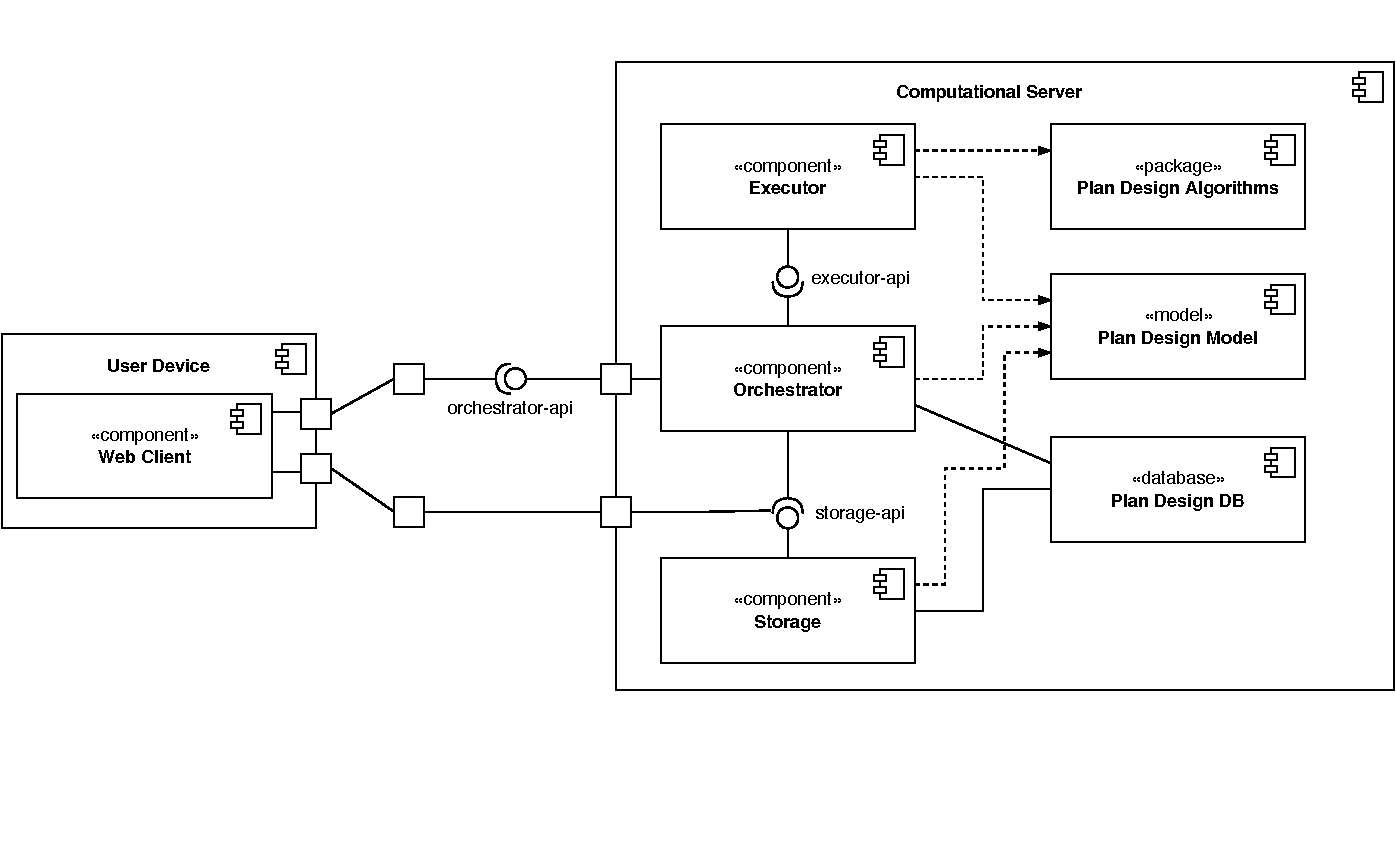
\includegraphics[width=\textwidth]{architecture/pictures/storage/component}
	\caption{Диаграмма компонент хранилища расчётных данных}
	\label{pic:architecture__storage-component}
\end{figure}
\vskip 5 mm


Сервис представлен следующими компонентами:
\begin{enumerate}
	\item {
		\textbf{API} -- отвечает за предоставление REST API и отправки задачи в очередь.
		\begin{itemize}
			\item \textit{Request Handler}
			\item \textit{Controller}
		\end{itemize}
	}
	\item {
		\textbf{Repository} -- отвечает за получение и сохранение данных и логику их преобразований.
		\begin{itemize}
			\item \textit{ModelRepository}
			\item \textit{FeatureRepository}
			\item \textit{GlossaryRepository}
		\end{itemize}
	}
	\item {
		\textbf{Data} -- преобразование сущностей базы данных в сущности модели данных.
		\begin{itemize}
			\item \textit{FeatureMapper}
			\item \textit{GlossaryMapper}
		\end{itemize}
	}
	\item {
		\textbf{Database} -- связь с базой данных.
		\begin{itemize}
			\item \textit{Database} -- обеспечение CRUD-операций для сущностей базы данных.
		\end{itemize}
	}
\end{enumerate}